
\chapter{Systementwurf}

In diesem Kapitel wird eine Entwurf für die Implementation des Systems aufgezeigt.
Die Struktur des Systems wird durch einen Architekturentwurf vorgegeben, wogegen eine Unschärfe bei der Implementation der Details erlaubt wird \todo{...rly? satz}.

Eine frühe Recherche hat ergeben, dass kein ASN.1 Compiler für Rust verfügbar ist.
Zwar sind einige Rust-Bibliotheken für ASN.1 zu finden (\textit{yasna}, \textit{raisin}, \textit{rust-asn1}, ...), jedoch kann keine UPER.
Keine der genannten Bibliotheken übersetzt, wie in der bisherigen Referenzimplementierung, die ASN.1 Datenstrukturen in native Datenstrukturen.
Auch keiner der von der ITU genannten Compiler\footnote{\url{https://www.itu.int/en/ITU-T/asn1/Pages/Tools.aspx}} unterstützen Rust .
Dieser Umstand erzwingt die Nutzung der C-Datenstrukturen der Referenzimplementierung mittels \gls{ffi} (siehe \autoref{rust:ffi}).
Zur besseren Kapselung ist die Einbindung der ASN.1 Nachrichten deswegen in mehreren Schritten in zwei Crates ausgelagert.

\todo{vorweg, kein ASN.1 Rust compiler, dh c bibliothek einbinden, unabhängigkeit von asn/nachrichtentechnologie weil sauber + weil schonmal wechsel von protobuf}

\section{Architektur / Komponentendiagramme}
		
In \autoref{draft:architecture} ist ein Entwurf der Architektur zu sehen.
Blau markierte Klassen haben als Aufgabengebiet die Kommunikation, grün markierte Klassen bilden die Geschäftslogik ab und rot markierte Klassen sind Spezialisierungen für ASN.1.


\begin{figure}[H]
	\centering
	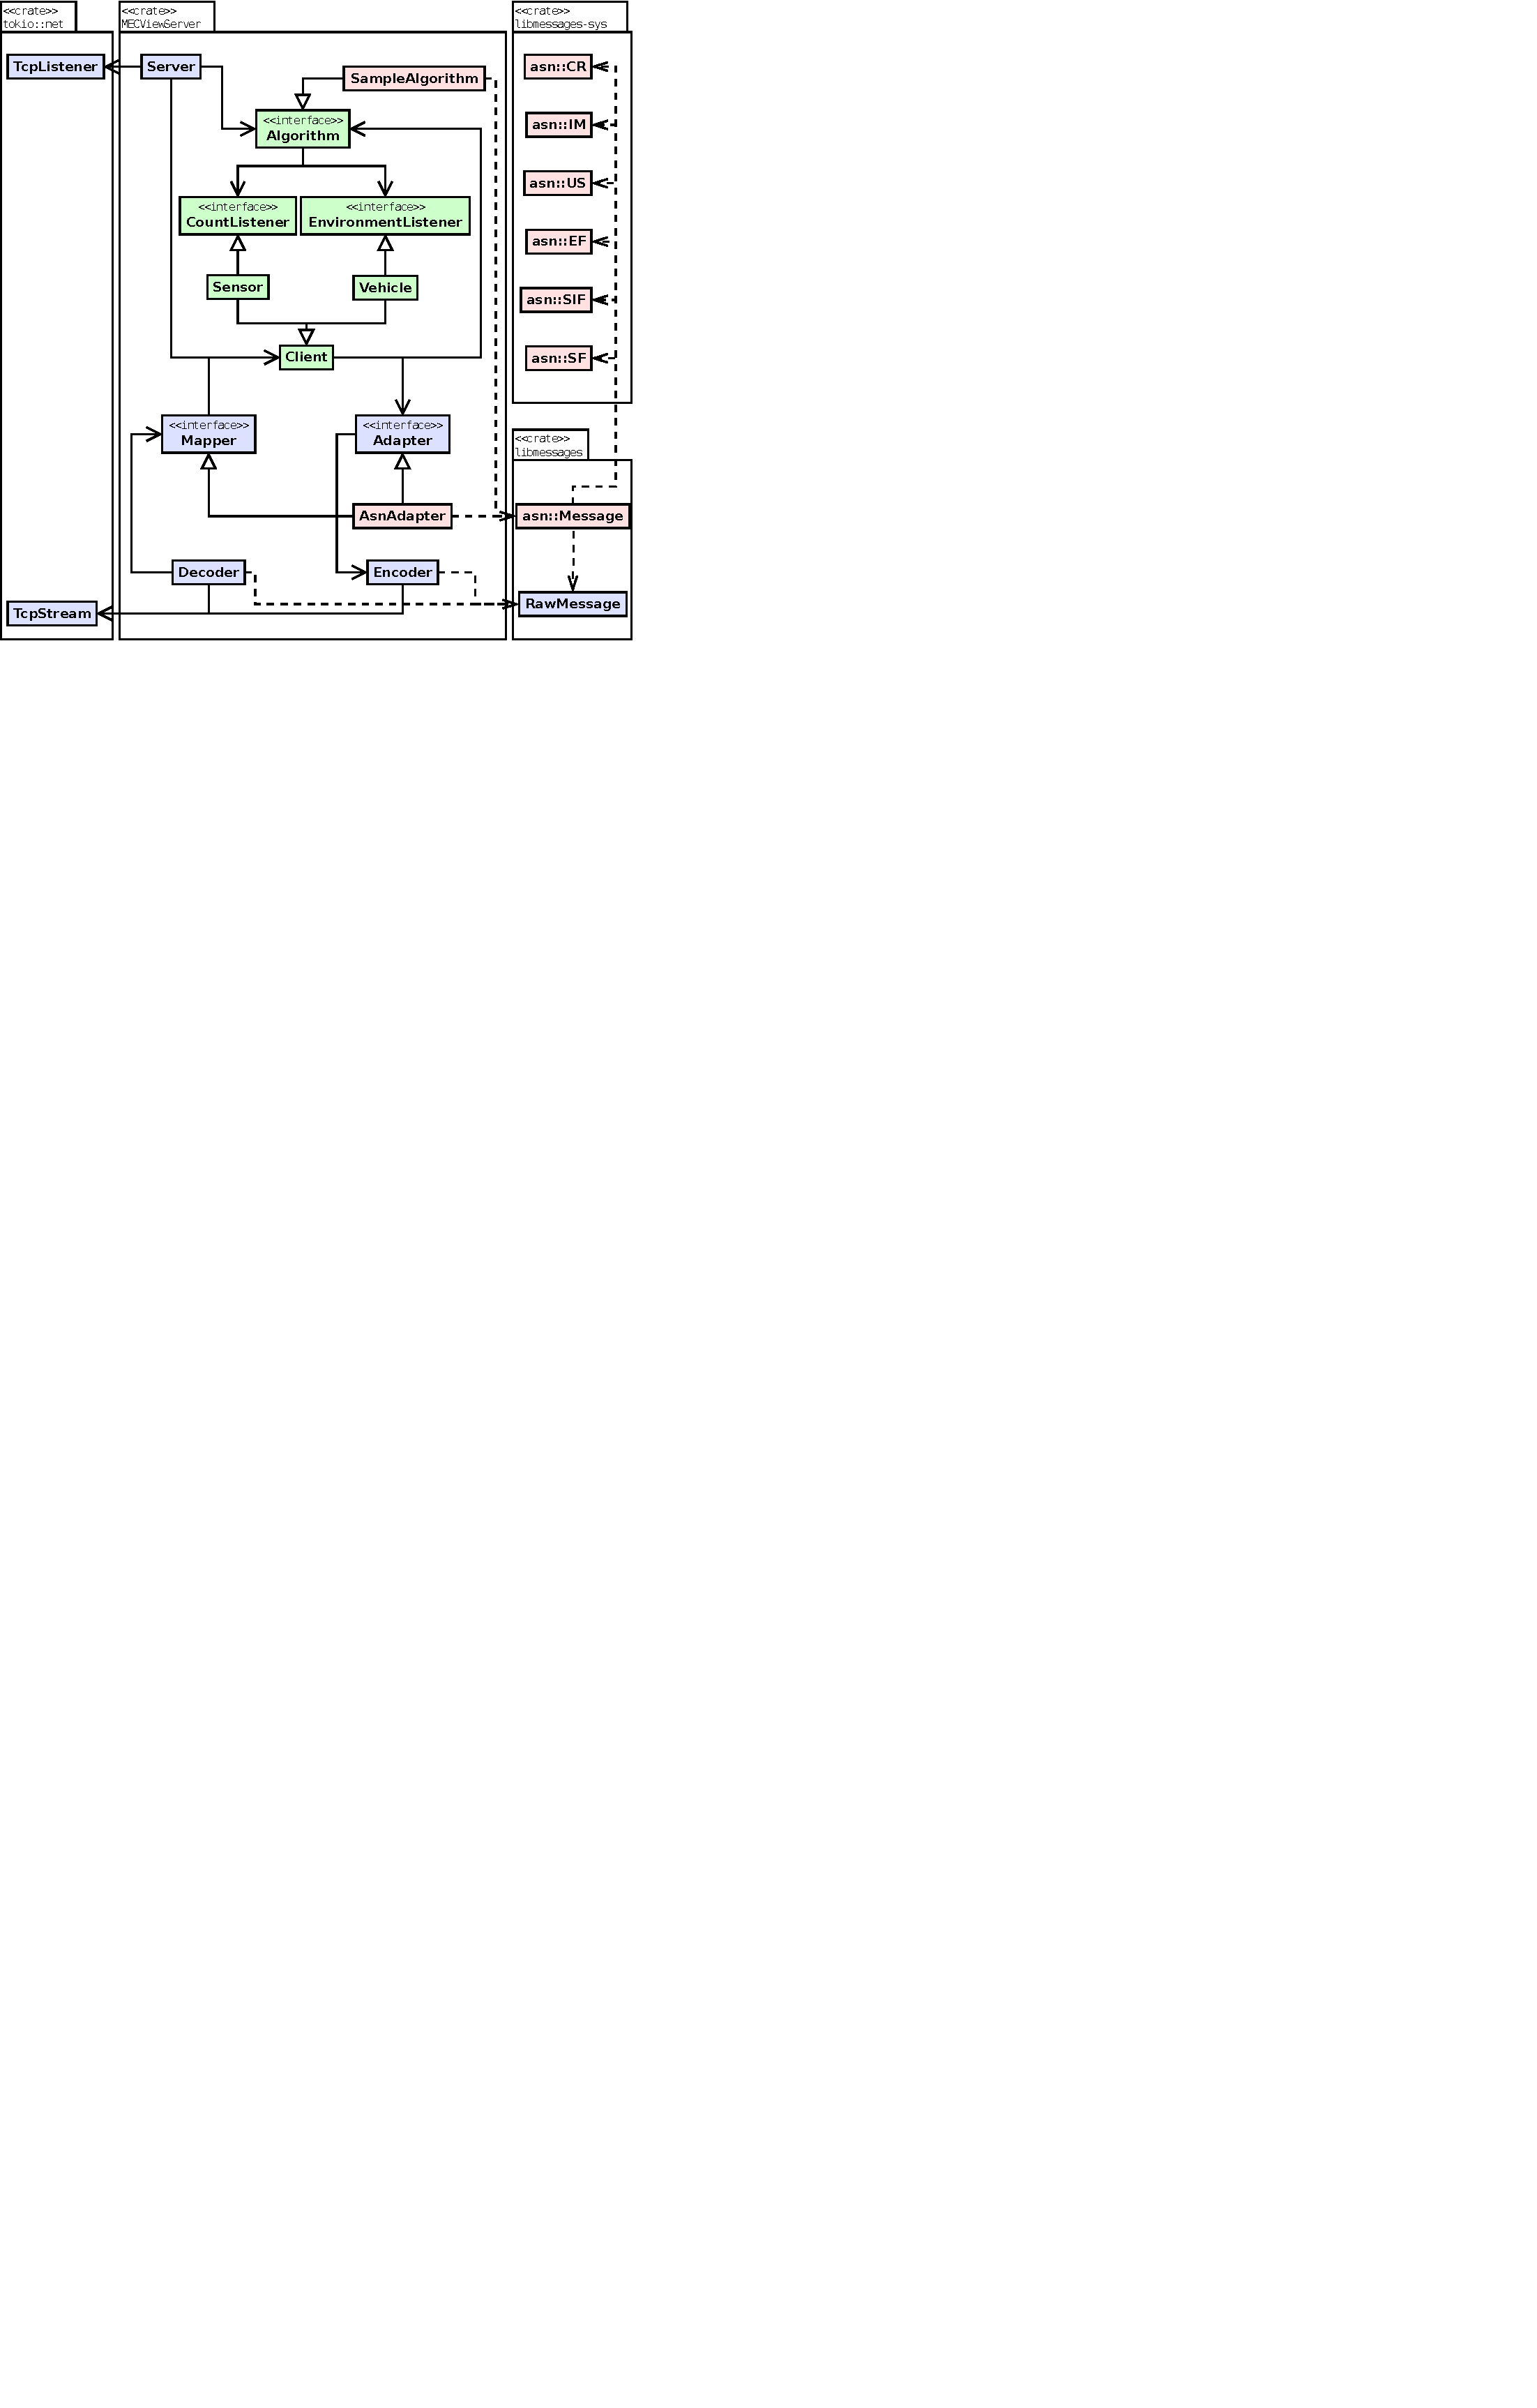
\includegraphics[width=2.0\textwidth]{dia/architecture}
	\caption{Architekturentwurf}
	\label{draft:architecture}
\end{figure}

Die Implementation soll in drei Crates aufgeteilt sein:
\begin{itemize}
	\item \textbf{libmessages-sys}: Soll bindings für die ASN.1 Datenstrukturen und Funktionen der C-Bibliothek beinhalten (siehe \autoref{rust:ffi}).
	Unsichere Funktionsaufrufe nach C, wie zur Serialisierung und Deserialisierung, sollen durch sichere Rust Funktionen gekapselt werden.
	Eine ordnungsgemäße Allokation und Deallokation der Nachrichten soll hier sichergestellt ermöglicht werden.
	
	\item \textbf{libmessages}: Soll Datenstrukturen und Implementationen bereit stellen um unabhängig von der eingesetzten Nachrichtentechnologie eine Nachricht abbilden zu können.
	Hierzu soll in \textit{RawMessage} der Kopf (siehe \autoref{analysis:messages}) und der binären Inhalt einer Nachricht dargestellt sein.
	
	Zusätzlich soll in dieser Crate für jede Verwendete Technologie (in dieser Bachelorarbeit nur ASN.1) die Wandlung zwischen einer \textit{RawMessage} und einer entsprechenden Datenstruktur implementiert werden.
	
	\item \textbf{MECViewServer}: Bündelt die Geschäfts- und Kommunikationslogik zu einem ausführbaren Kompilat.
\end{itemize}

\subsubsection{Erklärung Server}

Der Server lädt zu beginn eine Algorithmus Implementation, öffnet einen TCP-Port und wartet auf dem daraus resultierenden \textit{TcpListener} auf neue Clients.
Jedem neuen Client wird eine Referenz auf den Algorithmus mitgegeben.

\subsubsection{Erklärung Client, Sensor und Vehicle}

Der Client hält eine Referenz auf einen Algorithmus und einen Adapter.
Im Falle eines \textit{Vehicle}s kann ein \textit{EnvironmentListener} am Algorithmus registriert werden um neue Umgebungsmodelle zu erhalten.
Im Falle eines \textit{Sensor}s kann ein \textit{CountListener} am Algorithmus registriert werden um über Änderungen bei der Anzahl der registrierten Fahrzeuge informiert zu werden.

\subsubsection{Erklärung Adapter}

Der Adapter bietet eine Schnittstelle um damit eine Clientinstanz Nachrichten versenden kann, ohne die eingesetzte Nachrichtentechnologie zu kennen.
Hierzu sollen der Clientinstanz Funktionen bereitgestellt werden, die von der Adapterimplementation in entsprechende Nachrichten übersetzt werden.

\subsubsection{Erklärung Mapper}

Der Mapper ruft für Empfangene Nachrichten der eingesetzten Nachrichtentechnologie Funktionen der Clientinstanz auf und agiert somit als Gegenstück zum Adapter.

\subsubsection{Erklärung Encoder / Decoder}

Der Encoder soll \textit{RawMessage}s auf den TCP-Datenstrom schreiben, während der Encoder \textit{RawMessage}s vom TCP-Datenstrom lesen soll.
Hierzu muss eine Wandlung, wie in \autoref{analysis:messages} beschrieben, vorgenommen werden.

\subsubsection{Nachrichtentechnologie kapseln}

Innerhalb der MECViewServer Crate sollen möglichst wenige Klassen die eingesetzt Nachrichtentechnologie kennen.
Hierzu zählen die Algorithmus- (\textit{SampleAlgorithmus}), Mapper- und Adapterimplementationen (\textit{AsnAdapter}).
Dies ist unumgänglich, weil sowohl der eingesetzte Algorithmus, der Mapper und der Adapter Felder der Nachrichten lesen und schreiben müssen und dies voraussetzt, die Nachrichtentechnologie zu kennen.
Zudem muss der Server mindestens indirekt die eingesetzte Technologie kennen, um die richtigen und zueinander kompatiblen Algorithmus-, Mapper- und Adapterimplementation zu instantiieren.
Weitere Klassen sollen unabhängig von der eingesetzten Technologie agieren.

\subsection{Asynchrone Kommunikation}

Um ein Mehrkernsystem effizient zu nutzen, sollen einige Klassen asynchron zueinander arbeiten.
Hierzu zählt der Server, der asynchron zur Geschäftslogik neue Verbindungen annimmt.
Die daraus resultierenden Clientinstanzen sollen zum Server und zueinander asynchron ihre Anfragen bearbeiten.
Letztendlich soll auch der Algorithmus asynchron zu den Clients und dem Server das Umfeldmodell aktualisieren.


~\\ ~\\ ~\\






Ausgliederung von libmessages weil ASN-Bindings + weil von Protokolländerungen unabhängig sein soll

Prüfen tokio, queues, async + proxy pattern

Abbildung vereinfacht, Kommunikation via Queues im tokio context


\cite[446]{goll2012methoden}, example \cite[457]{goll2012methoden}

\todo{Component diagrams tikz-uml: server, algorithm, encoder/...}		

\section{Sequenzdiagramme}

\subsection{Low-Latency + Entwurfsmuster + Patterns? + Algorithmen?}
\todo{Hochperformant -> parallel?}

\todo{Design Pattern, Gamma et al, four important aspects}

\todo{Real Time Design Patterns Buch: Ab Seite 141, verschiedene Systempatterns, microkernel \cite[151]{douglass2003real}? channel architektur pattern \cite[167]{douglass2003real}?}

\todo{Message Queuing Pattern \cite[207]{douglass2003real}}

\todo{kein hartes Echtzeitsystem, gerade mal weiches Echtzeitsystem \autoref{real_time_system}}

\todo{Clean Architecture / Clean Code}